%%%%%%%%%%%%%%%%%%%%%%%%%%%%%%%%%%%%%%%%%%  不使用 authblk 包制作标题  %%%%%%%%%%%%%%%%%%%%%%%%%%%%%%%%%%%%%%%%%%%%%%
%-------------------------------PPT Title-------------------------------------
\title{18-晶格振动与第一原理分子动力学}
%-----------------------------------------------------------------------------
%----------------------------Author & Date------------------------------------

%\author[\textrm{Jun\_Jiang}]{姜\;\;骏\inst{}} %[]{} (optional, use only with lots of authors)
%% - Give the names in the same order as the appear in the paper.
%% - Use the \inst{?} command only if the authors have different
%%   affiliation.
%\institute[BCC]{\inst{}%
\institute[Gain~Strong]{\inst{}%
%\vskip -20pt 北京市计算中心}
\vskip -20pt {\large 格致斯创~科技}}
\date[\today] % (optional, should be abbreviation of conference name)
{%	{\fontsize{6.2pt}{4.2pt}\selectfont{\textcolor{blue}{E-mail:~}\url{jiangjun@bcc.ac.cn}}}
\vskip 45 pt {\fontsize{8.2pt}{6.2pt}\selectfont{%清华大学\;\;物理系% 报告地点
	\vskip 5 pt \textrm{2023.04.22}}}
}

%% - Either use conference name or its abbreviation
%% - Not really information to the audience, more for people (including
%%   yourself) who are reading the slides onlin%%   yourself) who are reading the slides onlin%%   yourself) who are reading the slides onlineee
%%%%%%%%%%%%%%%%%%%%%%%%%%%%%%%%%%%%%%%%%%%%%%%%%%%%%%%%%%%%%%%%%%%%%%%%%%%%%%%%%%%%%%%%%%%%%%%%%%%%%%%%%%%%%%%%%%%%%

\subject{}
% This is only inserted into the PDF information catalog. Can be left
% out.
%\maketitle
\frame
{
%	\frametitle{\fontsize{9.5pt}{5.2pt}\selectfont{\textcolor{orange}{“高通量并发式材料计算算法与软件”年度检查}}}
\titlepage
}
%-----------------------------------------------------------------------------

%------------------------------------------------------------------------------列出全文 outline ---------------------------------------------------------------------------------
%\section*{}
%\frame[allowframebreaks]
%{
%  \frametitle{Outline}
%%  \frametitle{\textcolor{mycolor}{\secname}}
%  \tableofcontents%[current,currentsection,currentsubsection]
%}
%%在每个section之前列出全部Outline
%%类似的在每个subsection之前列出全部Outline是\AtBeginSubsection[]
%\AtBeginSection[]
%{
%  \frame<handout:0>%[allowframebreaks]
%  {
%    \frametitle{Outline}
%%全部Outline中,本部分加亮
%    \tableofcontents[current,currentsection]
%  }
%}

%-----------------------------------------------PPT main Body------------------------------------------------------------------------------------
\small
%\section{\rm{VASP~}软件中\rm{PAW~}计算的实现}
%\frame
%
%	\frametitle{\textrm{VASP}计算的特色}
%	相比于与普通的第一原理计算软件,\textrm{VASP}很好地平衡了计算效率和精度的问题,总的来说,\textrm{VASP}主要通过这几个特色保证了计算的高效能
%	\begin{itemize}
%	     \item 迭代与优化算法的多样性\\
%		     本质上电荷密度迭代 \textrm{\&\&} 体系总能量优化是相同的优化问题,采用了类似的算法\upcite{CMS6-15_1996,PRB54-11169_1996}:\\
%			\textcolor{blue}{\textrm{Pseudo-Newton、Conjugate-Gradient、Broyden~mix、damping-factor、RMM-DIIS}}
%	     \item 尽可能采用局域基(原子轨道基)函数:~\\
%		     \textcolor{blue}{\textrm{LREAL}}=\textcolor{red}{\textrm{.TRUE.}}\\
%			优化的投影函数也尽可能在实空间表示
%	     \item \textrm{PAW}原子数据集:\textcolor{blue}{优异的赝势}\upcite{PRB59-1758_1999}
%	\end{itemize}
%}
\section{晶格振动与声子}
\subsection{晶格振动与简谐振动}
\frame
{
	\frametitle{简谐近似}
	\begin{itemize}
		\item 晶体中的格点表示原子的平衡位置,晶格振动是原子在格点附近的振动
		\item 红外、Raman光谱、中子衍射谱,热容、热导,电阻、超导和电-声耦合等都与晶格振动有关
		\item 绝热近似(\textrm{Born-Oppenheimer}近似)下,原子核是在电子总能量$E(\mathbf{R})$形成的势能面上运动
	\end{itemize}
	含有$N$个原子,平衡位置是$\mathbf{R}_i^0$,偏移位置矢量$\mathbf{\mu}_i(t)$,体系的势能函数在平衡位置作\textrm{Taylor~}级数展开
	\begin{displaymath}
%		\begin{aligned}
		V=V_0+\sum_{i=1}^{3N}\left( \frac{\partial V}{\partial \mu_i} \right)_0\mu_i+\underline{\textcolor{red}{\frac12\sum_{i,j=1}^{3N}\left( \frac{\partial^2V}{\partial\mu_i\partial\mu_j} \right)_0\mu_i\mu_j}}+\mbox{高阶项}
%		\end{aligned}
	\end{displaymath}
	平衡位置$\left( \frac{\partial V}{\partial\mu_i} \right)_0=0$,\textcolor{blue}{简谐近似}保留到$\mu_i$的二次项
}

\frame
{
	\frametitle{简正坐标与简谐振动}
	$N$原子体系的动能函数
	\begin{displaymath}
		T=\frac12\sum_{i=1}^{3N}m_i\dot{\mu}_i^2
	\end{displaymath}
	引入简正坐标,\textcolor{blue}{与原子位移坐标$\mu_i$正交变换}
	\begin{displaymath}
		\sqrt{m_i}\mu_i=\sum_{j=1}^{3N}a_{ij}Q_j
	\end{displaymath}
	\textcolor{red}{目的}:~系统的势能函数与动能函数有简单形式(只有平方项)
	\begin{displaymath}
%		\begin{aligned}
			T=\frac12\sum_{i=1}^{3N}\dot{Q}_i^2\quad
			V=\frac12\sum_{i=1}^{3N}\omega_i^2Q_i^2
%		\end{aligned}
	\end{displaymath}
	由此可得谐振方程
	\begin{displaymath}
		\ddot{Q}_i+\omega_i^2Q_i=0\quad i=1,2,3,\cdots,3N
	\end{displaymath}

}

\frame
{
	\frametitle{简谐振动与振动模式}
	任意简正坐标解
	\begin{displaymath}
		Q_i=A\sin(\omega_it+\delta)
	\end{displaymath}
	由此得到原子位移坐标
	\begin{displaymath}
		\mu_i=\frac{a_{ij}}{\sqrt{m_i}}A\sin(\omega_it+\delta)
	\end{displaymath}
\begin{figure}[h!]
\centering
%\hspace*{-10pt}
\vspace*{-0.1in}
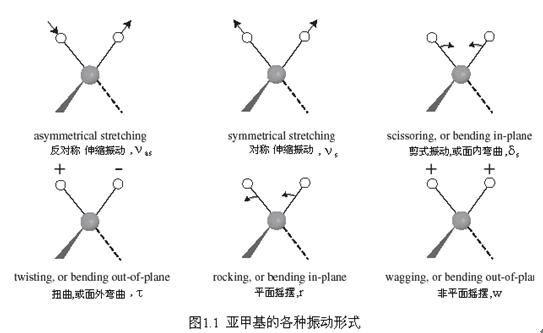
\includegraphics[height=1.in,width=2.in,viewport=0 20 420 250,clip]{Figures/RF_vir.jpg}
\caption{\tiny \textrm{Schematic example of vibration model of dimethyl.}}%
\label{virbration_model}
\end{figure} 
\textcolor{red}{简谐振动不表示某个原子的振动,表示整个体系所有原子参与的振动。这种体系中所有原子一起参加的共同振动常称为振动模}
}

\frame
{
	\frametitle{一维单原子链}
\begin{figure}[h!]
\centering
%\hspace*{-10pt}
\vspace*{-0.25in}
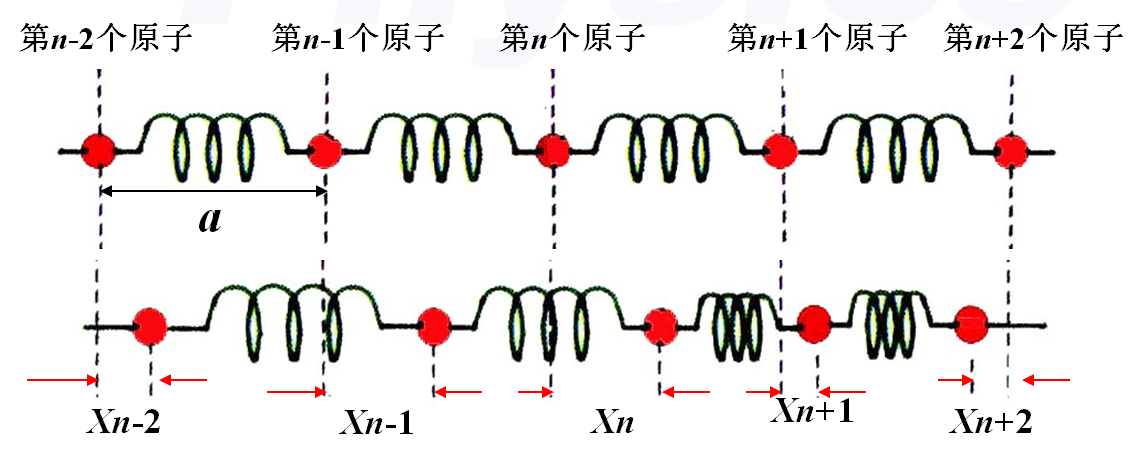
\includegraphics[height=1.0in,width=2.8in,viewport=0 0 1400 500,clip]{Figures/virbration.png}
\caption{\tiny \textrm{Schematic example of vibration of 1D-atomic chain.}}%
\label{virbration}
\end{figure} 
单原子链可以视为最简单的晶格,平衡时相邻原子距离为$\mathbf{a}$,原子限制在沿链方向运动,偏离格点位置用$\cdots,\mathbf{X}_{n-1},\mathbf{X}_{n},\mathbf{X}_{n+1},\cdots$,原子的振动可以表示为
\begin{displaymath}
	\mu_{nq}=A\mathrm{e}^{\mathrm{i}(\omega t-qx)}
\end{displaymath}
其中振幅$A$是常数,$\omega$是圆频率,$q=\tfrac{2\pi}{\lambda}$是波数,$\lambda$是波长\\
\textcolor{blue}{根据量子理论,每种简谐振动的能量是量子化的,可以用声子表示}
\begin{displaymath}
	\varepsilon_{nq}=\left( n+\frac12 \right)\hbar\omega_q
\end{displaymath}
}

\frame
{
	\frametitle{双原子链与光学支和声学支}
\begin{figure}[h!]
\centering
%\hspace*{-10pt}
\vspace*{-0.25in}
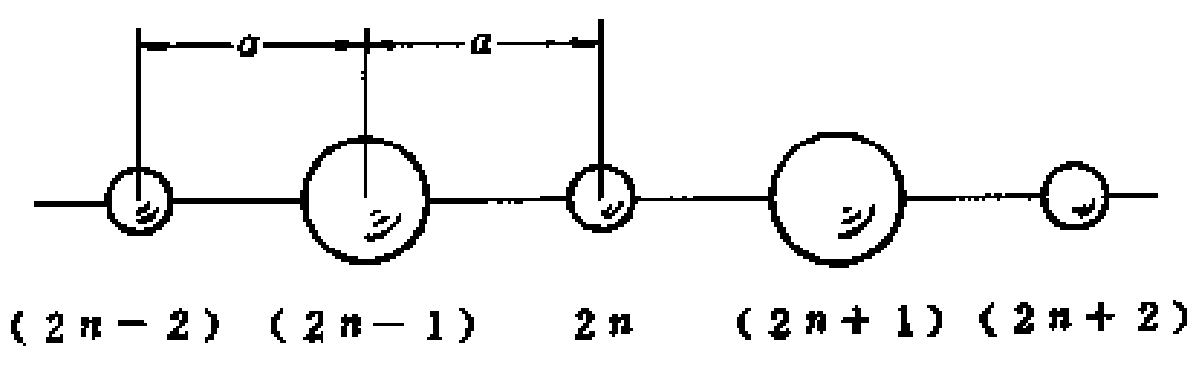
\includegraphics[height=0.7in,width=2.6in,viewport=0 0 1400 400,clip]{Figures/virbration-2.png}
\caption{\tiny \textrm{Schematic example of vibration of 1D-diatomic chain.}}%
\label{virbration-2D}
\end{figure} 
一维双原子链是最简单的复式晶格,平衡时相邻原子间距为$\mathbf{a}$,每个原胞含有两个不同原子\textrm{P}和\textrm{Q}质量分别是$m$和$M$,原子现在在沿链方向运动,偏离位移用$\cdots,\mu_{2n},\mu_{2n+1},\cdots$\\原子的运动方程
\begin{displaymath}
	\begin{aligned}
		&\mbox{\textrm{P}原子:~}m\ddot{\mu}_{2n}=-\beta(2\mu_{2n}-\mu_{2n+1}-\mu_{2n-1})\\
		&\mbox{\textrm{Q}原子:~}M\ddot{\mu}_{2n+1}=-\beta(2\mu_{2n+1}-\mu_{2n+2}-\mu_{2n})
	\end{aligned}
\end{displaymath}
可得关于振动频率$\omega$的两组解
\begin{displaymath}
	\omega^2\left.
	\begin{aligned}
		&\nearrow\omega_+^2\\
		&\searrow\omega_-^2
	\end{aligned}\right\}
	=\beta\frac{m+M}{mM}\left\{ 1\pm\left[ 1-\frac{4mM}{(m+M)^2}\sin^2aq \right]^{1/2} \right\}
\end{displaymath}
}

\frame
{
	\frametitle{光学支和声学支的长波极限}
\begin{figure}[h!]
\begin{minipage}[t]{0.3\linewidth}
\centering
\vspace*{-0.3in}
%\hspace*{-10pt}
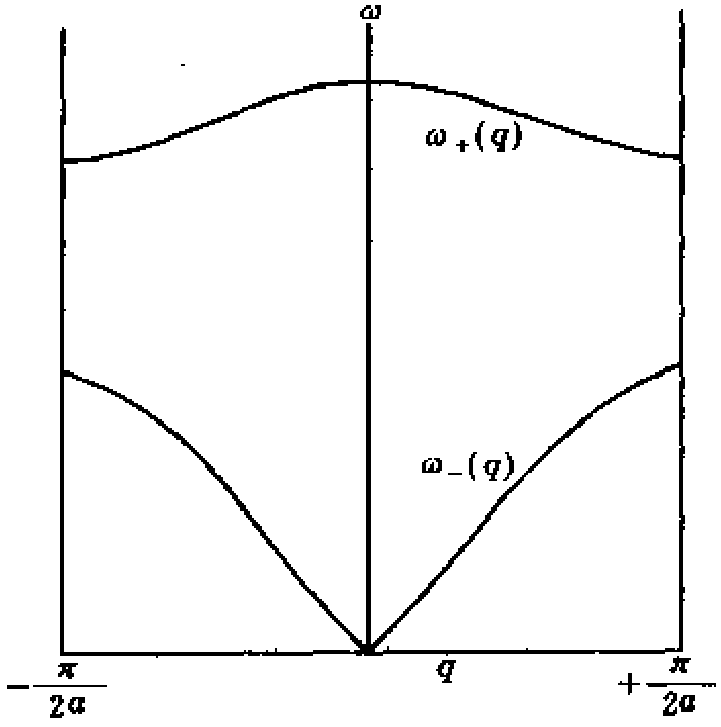
\includegraphics[height=1.in,width=1.in,viewport=0 0 700 800,clip]{Figures/Optic-Acous.png}
\label{optic_acous}
\end{minipage}
\hfill
\begin{minipage}[t]{0.67\linewidth}
%\vspace*{-0.3in}
	\begin{itemize}
		\item \textcolor{blue}{光学支}:~属于频率$\omega_+$的晶格简谐振动
		\item \textcolor{blue}{声学支}:~属于频率$\omega_-$的晶格简谐振动
	\end{itemize}
\end{minipage}
\caption{\tiny \textrm{The acoustic branch and optical branch.}}%
\end{figure} 
声学支的长波极限($q\rightarrow0$):
\begin{displaymath}
	\omega_-\approx a\sqrt{\frac{2\beta}{m+M}}q\quad\mbox{\textcolor{blue}{一维链看成连续介质的弹性波}}
\end{displaymath}
光学支的长波极限($q\rightarrow0$):
\begin{displaymath}
	\omega_+\approx a\sqrt{\frac{2\beta}{\left( \frac{mM}{m+M} \right)}}\quad\mbox{\textcolor{blue}{两种原子具有相反的相位,质心保持不动}}
\end{displaymath}
}

\frame
{
	\frametitle{经典三维振动模式}
			位于$\mathbf{R}_I(t)$的原子核运动的经典力学描述
			\begin{displaymath}
				M_I\frac{\partial^2\mathbf{R}_I}{\partial t^2}=\vec F_I(\mathbf{R})=-\frac{\partial}{\partial\mathbf{R}_I}E(\mathbf{R})
			\end{displaymath}
			晶格平衡位置$\{\mathbf{R}_I^0\}=\mathbf R^0$由原子核受力平衡确定
			\begin{displaymath}
				\vec F_I(\mathbf R^0)=0
			\end{displaymath}
			\textcolor{blue}{对平衡位置偏移的受力方程为}
			\begin{displaymath}
				C_{I,\alpha;J,\beta}=\frac{\partial^2E(\mathbf{R})}{\partial\mathbf{R}_{I,\alpha}\partial\mathbf{R}_{J,\beta}}
			\end{displaymath}
			其中$\alpha,\beta\cdots$是\textrm{cartesian}坐标

			\textcolor{blue}{谐振子近似下},频率为$\omega$的谐振模式下,晶格对平移位置的偏移为
			\begin{displaymath}
				\mathbf{u}_I(t)=\mathbf{R}_I(t)-\mathbf{R}_I^0\equiv\mathbf{u}_I\mathrm{e}^{\mathrm{i}\omega t}
			\end{displaymath}
			对位于$I$的原子核(质量为$M_I$),有
			\begin{displaymath}
				-\omega^2M_Iu_{I\alpha}=-\sum_{J\beta}C_{I,\alpha;J\beta}u_{J\beta}
			\end{displaymath}
			因此振动频率$\omega$,由经典谐振方程确定
			\begin{displaymath}
				\det\left|\frac1{\sqrt{M_IM_J}}C_{I,\alpha;J\beta}-\omega^2\right|=0
			\end{displaymath}
}

\frame
{
	\frametitle{晶格振动模式(冻声子方法)}
	对于周期性的晶格振动,根据\textrm{Bl\"och~}定理,振动引起的位置偏移
			\begin{displaymath}
				\mathbf{u}_s(\vec T_n)\equiv\mathbf{R}_s(\vec T_n)-\mathbf{R}_s^0(\vec T_n)=\mathrm{e}^{\mathrm{i}\vec k\cdot\vec T_n}\mathbf{u}_s(\vec k)
			\end{displaymath}
			由此得谐振方程
			\begin{displaymath}
				\det\left|\frac1{\sqrt{M_sM_{s^{\prime}}}}C_{s,\alpha;s^{\prime}\alpha^{\prime}}-\omega_{i\vec k}^2\right|=0
			\end{displaymath}
			这里原子标记$s=1,S$,对应的谐振模式$i=1,3S$

			每个$\vec k$的约化力常数矩阵可表示为
			\begin{displaymath}
				\begin{aligned}
				C_{s,\alpha;s^{\prime}\alpha^{\prime}}(\vec k)=&\sum_{\vec T_n}\mathrm{e}^{\mathrm{i}\vec k\cdot\vec T_n}\frac{\partial^2 E(\mathbf{R})}{\partial\mathbf{R}_{s,\alpha}(0)\partial\mathbf{R}_{s^{\prime},\alpha^{\prime}}(\vec T_n)}\\
				=&\frac{\partial^2E(\mathbf{R})}{\partial\mathbf{u}_{s,\alpha}(\vec k)\partial\mathbf{u}_{s^{\prime},\alpha^{\prime}}(\vec k)} 
				\end{aligned}
			\end{displaymath}
}

\subsection{绝热近似与电-声耦合}
\frame
{
	\frametitle{绝热近似}
	绝热近似(\textrm{Born-Oppenheimer~}近似)下,忽略原子核动能的运动,电子的本征态(本征值$E_i\{\mathbf{R}\}$,波函数$\Psi_i(\{\mathbf{r}\}:\{\mathbf{R}\})$)中原子核坐标是$\{\mathbf{R}\}$参数

	如果考虑核与电子体系,\textrm{Hamiltonian~}算符可以写成
	\begin{displaymath}
		\hat H=\hat T_N+\hat T_e+\hat U
	\end{displaymath}
	$U$是全部相互作用,可由\textcolor{blue}{电子坐标$\{\mathbf{r}\}$}和\textcolor{blue}{原子核坐标$\{\mathbf{R}\}$}表示

	核与电子耦合体系的完全解是
	\begin{displaymath}
		\hat H\Psi_s(\{\mathbf{r},\mathbf{R}\})=E_s\Psi_s(\{\mathbf{r},\mathbf{R}\})
	\end{displaymath}
	这里$s=1,2,3,\cdots$

	如果对于原子核位于$\{\mathbf{R}\}$的电子态是$\Psi_i(\{\mathbf{r}\}:\{\mathbf{R}\})$
	\begin{displaymath}
		\Psi(\{\mathbf{r},\mathbf{R}\})=\sum_i\chi_{si}(\{\mathbf{R}\})\Psi_i(\{\mathbf{r}\}:\{\mathbf{R}\})
	\end{displaymath}
}

\frame
{
	\frametitle{绝热近似}
	包含电子-原子核耦合的$\chi_{si}(\{\mathbf{R}\})$运动方程
	\begin{displaymath}
		[T_N+E_i(\{\mathbf{R}\})-E_s]\chi_{si}(\{\mathbf{R}\})=-\sum_{ii^{\prime}}C_{ii^{\prime}}\chi_{si}(\{\mathbf{R}\})
	\end{displaymath}
	这里$T_n=-\frac12(\sum\limits_J\nabla_J^2/M_J)$,矩阵元$C_{ii^{\prime}}=A_{ii^{\prime}}+B_{ii^{\prime}}$
	\begin{displaymath}
		\begin{aligned}
			A_{ii^{\prime}}(\{\mathbf{R}\})=&\sum_J\frac1{M_J}\langle\Psi_i(\{\mathbf{r}\}:\{\mathbf{R}\})|\nabla_J|\Psi_{i^{\prime}}(\{\mathbf{r}\}:\{\mathbf{R}\})\rangle\nabla_J\\
			B_{ii^{\prime}}(\{\mathbf{R}\})=&\sum_J\frac1{2M_J}\langle\Psi_i(\{\mathbf{r}\}:\{\mathbf{R}\})|\nabla_J^2|\Psi_{i^{\prime}}(\{\mathbf{r}\}:\{\mathbf{R}\})\rangle\\
		\end{aligned}
	\end{displaymath}
	这里$\langle\Psi_i(\{\mathbf{r}\}:\{\mathbf{R}\})|\hat O|\Psi_{i^{\prime}}(\{\mathbf{r}\}:\{\mathbf{R}\})\rangle$表示对电子变量$\{\mathbf{r}\}$积分
}

\frame
{
	\frametitle{绝热近似}
	绝热近似下,\textcolor{red}{将忽略矩阵$C_{ii^{\prime}}$的全部非对角元},可有
	\begin{itemize}
		\item \textcolor{blue}{电子能及时响应原子核的运动}
		\item \textcolor{blue}{电子由态$i\rightarrow i^{\prime}$的激发,不会影响原子核位置变量${\{\mathbf{R}\}}$}
		\item $A_{ii^{\prime}}=0$(波函数归一化要求)
		\item 核运动的势函数$U_i(\{\mathbf{R}\})=E_i(\{\mathbf{R}\})+B_{ii}(\{\mathbf{R}\})$
	\end{itemize}
	核运动方程运动方程
	\begin{displaymath}
		\left[ -\sum_J\frac1{2M_J}\nabla_J^2+U_i(\{\mathbf{R}\})-E_{ni} \right]\chi_{ni}(\{\mathbf{R}\})=0
	\end{displaymath}
这里$n=1,2,3,\cdots$

如果忽略$B_{ii}$的贡献,即冻声子近似(\textrm{frozen phonon})或微扰方法
}

\frame
{
	\frametitle{电-声耦合}
	电子-声子的来源:~\textcolor{blue}{$C_{ii^{\prime}}$的非对角元部分}
	\begin{itemize}
		\item $C_{ii^{\prime}}$的非对角元部分描述了\textcolor{red}{原子核运动(振动)引起电子在不同态间跃迁}
		\item $C_{ii^{\prime}}$的非对角元部分主要来自$A_{ii^{\prime}}$
			\begin{enumerate}
				\item 电子波函数$\Psi_i(\{\mathbf{r}\}:\{\mathbf{R}\})$对原子核位置$\{\mathbf{Rj}\}$的梯度
				\item 梯度算符对声子波函数$\chi_{si}(\{\mathbf{R}\})$的贡献
			\end{enumerate}
		\item 电子在态$i\rightarrow i^{\prime}$跃迁将会激发或吸收一个声子
	\end{itemize}
	线性近似下有
	\begin{displaymath}
		\hspace*{-15pt}
		\langle\Psi_i(\{\mathbf{r}\}:\{\mathbf{R}\})|\nabla_J|\Psi_i^{\prime}(\{\mathbf{r}\}:\{\mathbf{R}\})\rangle=\frac{\langle\Psi_i(\{\mathbf{r}\}:\{\mathbf{R}\})|\tfrac{\nabla_V}{\nabla_{\mathbf{R}_J}}|\Psi_{i^{\prime}}(\{\mathbf{r}\}:\{\mathbf{R}\})\rangle}{E_{i^{\prime}}(\{\mathbf{R}\})-E_i(\{\mathbf{R}\})}
	\end{displaymath}
}

\section{第一原理分子动力学}
\frame
{
	\frametitle{第一原理分子动力学\textrm{AIMD}}
	1985年\textrm{Car}和\textrm{Parrinello}在密度泛函理论基础上,将第一原理方法应用到分子动力学研究中,形成第一原理分子动力学\textrm{(Ab~initio Molecular dynamics, AIMD)}
	\begin{itemize}
		\item \textrm{AIMD}将电子结构与原子和经典轨迹计算在同一基础上完成
		\item 每个原子运动步的受力都是在电子结构计算基础上获得的
		\item 基于\textrm{B-O}近似,原子运动径迹的每一步上,电子运动都达到收敛
		\item 扩展的\textrm{Lagrangian}方法:~根据体系几何结构变化构造体系波函数\\
			\textrm{Car-Parinello}:~平面波基,构成分子轨道
			\textrm{ADMP}:~原子中心基,构成密度矩阵
	\end{itemize}
	\textrm{AIMD}计算内容
	\begin{itemize}
		\item 可用于复杂体系的电子结构计算
		\item 几何结构优化(能量最小化)
		\item 描述系统演化
		\item 模拟时长达到$\approx{\mathrm{ps}}$~(经典分子动力学 $\approx\mathrm{ns}$)
	\end{itemize}

}


